%=====================================================================
%  CADENCE — IEEE ICA 2026 (IEEEtran conference), target 6 pages
%  Compile on Overleaf: pdfLaTeX (single file; bibliography is inline).
%  Figures in ./figures. Every quantitative claim is measured; unrun
%  experiments are stated as limitations, never as results.
%  References are listed in ASCENDING order of publication year.
%=====================================================================
\documentclass[conference]{IEEEtran}
\IEEEoverridecommandlockouts
\usepackage{cite}
\usepackage{amsmath,amssymb,amsfonts}
\usepackage{graphicx}
\usepackage{booktabs}
\usepackage{array}
\usepackage{pifont}
\usepackage{textcomp}
\usepackage{xcolor}
\usepackage[hidelinks]{hyperref}
\graphicspath{{figures/}}
\newcommand{\yes}{\ding{51}}
\newcommand{\no}{\textcolor{gray}{\ding{55}}}

\begin{document}

\title{CADENCE: Causal Drift Attribution and\\ Cost-Constrained Retraining for Continually\\ Deployed Machine-Learning Systems%
\thanks{CSE: Computer Science and Engineering; LPU: Lovely Professional University, India.}}

\author{%
\IEEEauthorblockN{Gona Lalith}\IEEEauthorblockA{Dept.\ of CSE, LPU\\ Phagwara, India\\ gonalalith2005@gmail.com}
\and
\IEEEauthorblockN{Ankita Maji}\IEEEauthorblockA{Dept.\ of CSE, LPU\\ Phagwara, India\\ ankitamaji7033@gmail.com}
\and
\IEEEauthorblockN{Nihar Kanakam}\IEEEauthorblockA{Dept.\ of CSE, LPU\\ Phagwara, India\\ niharkanakam@gmail.com}
\\[1ex]
\IEEEauthorblockN{Quaise Mallick}\IEEEauthorblockA{Dept.\ of CSE, LPU\\ Phagwara, India\\ quaisemallick.wha@gmail.com}
\and
\IEEEauthorblockN{Shailaja Singh}\IEEEauthorblockA{Dept.\ of CSE, LPU\\ Phagwara, India\\ sshailaja2004@gmail.com}
\and
\IEEEauthorblockN{Jasmeen Khatun}\IEEEauthorblockA{Dept.\ of CSE, LPU\\ Phagwara, India\\ jasmeenkhatun536@gmail.com}
\and
\IEEEauthorblockN{Dr.\ Ravin Kumar}\IEEEauthorblockA{School of CSE, LPU\\ Punjab, India\\ ravinpal2009@gmail.com}
}

\maketitle

\begin{abstract}
Deployed machine-learning models degrade as data distributions drift, yet the
dominant maintenance policies---periodic and drift-triggered full
retraining---answer only \emph{when} to retrain, never \emph{which} part of the
model failed or \emph{how much} of it to repair. We present CADENCE, a
closed-loop framework that (i) builds a drift-attribution graph over external
input features \emph{and} internal activation clusters, (ii) scores per-node
responsibility with a graph neural network and predicts each repair's benefit
with a counterfactual surrogate, and (iii) selects a minimal, cost- and
SLA-constrained retraining scope. Under a pre-registered protocol in which we
report negative results as first-class findings, the learned attribution beats
a Population-Stability-Index baseline on contested synthetic drift (mean
reciprocal rank $0.10{\to}0.41$, AUROC $0.67{\to}0.91$; $p<0.001$, $n{=}10$);
targeted partial retraining cuts Split-MNIST forgetting from $39.5\%$ to near
zero against a fair replay baseline ($p<0.001$, $n{=}10$); and on real
electricity-market drift the policy saves $69.1\%$ of retraining compute for a
$1.66$-point F1 cost. We further show, honestly, that the framework is
net-positive only above a measured retrain-cost break-even, that graph
construction scales as $\approx O(n^{2.6})$, and that a learned policy is
competitive-but-not-superior to a greedy rule at a three-action scale---defining
the operating envelope of diagnosis-driven model repair.
\end{abstract}

\begin{IEEEkeywords}
concept drift, causal attribution, graph neural networks, constrained
reinforcement learning, continual learning, MLOps.
\end{IEEEkeywords}

%=====================================================================
\section{Introduction}
%=====================================================================
A model that is accurate at deployment does not stay accurate: as the serving
distribution drifts, quality erodes, and the effort of a deployed ML system is
spent largely \emph{after} first training~\cite{sculley2015,paleyes2022}. Two
responses dominate practice. \emph{Periodic} retraining refits on a calendar,
paying compute whether or not anything changed; \emph{reactive} retraining fires
a full refit when a drift alarm crosses a threshold. Both treat the model as a
black box and decide only \emph{when} to retrain---never \emph{which component
failed} or \emph{how much to repair}. A covariate shift in one feature and a
wholesale concept change demand very different responses, yet both trigger the
same expensive full retrain, and a naive full retrain can induce catastrophic
forgetting~\cite{mccloskey1989} of previously served sub-populations.

We argue the right unit of decision is \emph{minimum-cost repair under a
performance constraint}: given a degradation, attribute it across the
input--model system, estimate the benefit of a candidate repair, and execute the
smallest intervention that restores service within a service-level agreement
(SLA). This reframes maintenance as a causal-attribution problem feeding a
constrained sequential decision.

\textbf{Contributions.} (1) A hybrid causal drift-attribution graph (CDAG)
spanning external features and internal activation clusters, with a learned GNN
readout that beats correlation where the problem is hard (Sec.~\ref{sec:h1}).
(2) A counterfactual surrogate that predicts repair benefit ($R^2{=}0.89$) and an
honest analysis of its out-of-distribution failure (Sec.~\ref{sec:sur}). (3) A
cost/SLA-constrained retraining-scope selector, with a pre-registered diagnostic
that the learned policy is non-degenerate---and a measured finding that it is not
superior to a greedy rule at this scale (Sec.~\ref{sec:h2},~\ref{sec:sys}). (4) A
pre-registered, reproducibility-first evaluation across synthetic and real drift
and three model families in which negatives are reported (Sec.~\ref{sec:res}).

%=====================================================================
\section{Related Work (Chronological)}\label{sec:rw}
%=====================================================================
Catastrophic interference in connectionist networks was identified
early~\cite{mccloskey1989}. Constraint-based causal structure discovery
matured with the PC algorithm~\cite{spirtes2000}, and error-rate drift
detectors such as DDM~\cite{gama2004} established the trigger-on-degradation
pattern later surveyed comprehensively~\cite{gama2014}. Production concerns were
crystallized as hidden technical debt~\cite{sculley2015}. A wave of learning
machinery followed: elastic weight consolidation (EWC) for
forgetting~\cite{kirkpatrick2017}, gradient-episodic memory~\cite{lopezpaz2017},
proximal policy optimization (PPO) for control~\cite{schulman2017}, inductive
graph representation learning~\cite{hamilton2017,kipf2017}, and Shapley-value
feature attribution~\cite{lundberg2017}. Continuous causal-structure learning
was made differentiable by NOTEARS~\cite{zheng2018}, while the preregistration
movement argued for fixing hypotheses before analysis~\cite{nosek2018}. Concept
drift was re-reviewed for the deep era~\cite{lu2019} and dataset-shift detectors
were studied empirically~\cite{rabanser2019}. Recent work consolidated reliable
RL implementations~\cite{raffin2021}, surveyed continual
learning~\cite{delange2022}, and catalogued the practical challenges of
deploying ML~\cite{paleyes2022}.

\emph{Positioning.} Drift detectors answer \emph{whether} the input moved;
causal discovery targets graph \emph{recovery}; continual learning supplies
update \emph{mechanisms}; attribution explains \emph{predictions}, not
degradation; and cost-aware retraining decides \emph{timing}. CADENCE instead
\emph{couples diagnosis to repair scope}: an attribution graph over external and
internal state, a learned estimate of each repair's benefit, and a
cost-constrained choice of \emph{how much} to retrain. We do not claim novelty
from the components individually; Table~\ref{tab:matrix} makes the system-level
distinction falsifiable.

\begin{table}[t]
\centering\footnotesize
\caption{Capability comparison against representative prior families. A mark
denotes a designed, first-class capability.}
\label{tab:matrix}
\setlength{\tabcolsep}{3.5pt}
\begin{tabular}{@{}lcccccc@{}}
\toprule
\textbf{Method} & \textbf{Drift} & \textbf{Attrib.} & \textbf{Internal} & \textbf{Counterf.} & \textbf{Scope} & \textbf{Cost/SLA}\\
\midrule
Drift detect.~\cite{gama2004,rabanser2019} & \yes & \no & \no & \no & \no & \no\\
Causal disc.~\cite{spirtes2000,zheng2018} & \no & \yes & \no & varies & \no & \no\\
Continual~\cite{kirkpatrick2017,lopezpaz2017} & \no & \no & \no & \no & \yes & \no\\
Attribution~\cite{lundberg2017} & \no & \no & \no & \no & \no & \no\\
Triggered retrain & \yes & \no & \no & \no & varies & varies\\
\textbf{CADENCE} & \yes & \yes & \yes & \yes & \yes & \yes\\
\bottomrule
\end{tabular}
\end{table}

%=====================================================================
\section{The CADENCE Framework}\label{sec:method}
%=====================================================================
Fig.~\ref{fig:arch} shows the closed loop. \emph{Monitor}: a privacy-filtered
collector samples feature windows and internal activations and runs a
PSI + delayed-label F1 trigger. \emph{Attribute}: on an alert a CDAG is built
over feature nodes and per-layer activation-cluster nodes using PC for the
skeleton~\cite{spirtes2000} and a NOTEARS-style continuous
relaxation~\cite{zheng2018} for weights; a GraphSAGE/GCN
readout~\cite{hamilton2017,kipf2017} yields node embeddings. \emph{Decide}: a
retraining-scope optimizer selects an action. \emph{Repair}: an executor applies
an EWC-regularized~\cite{kirkpatrick2017} partial or full retrain, then
shadow/canary validation promotes or rolls back.

\begin{figure}[t]
\centering
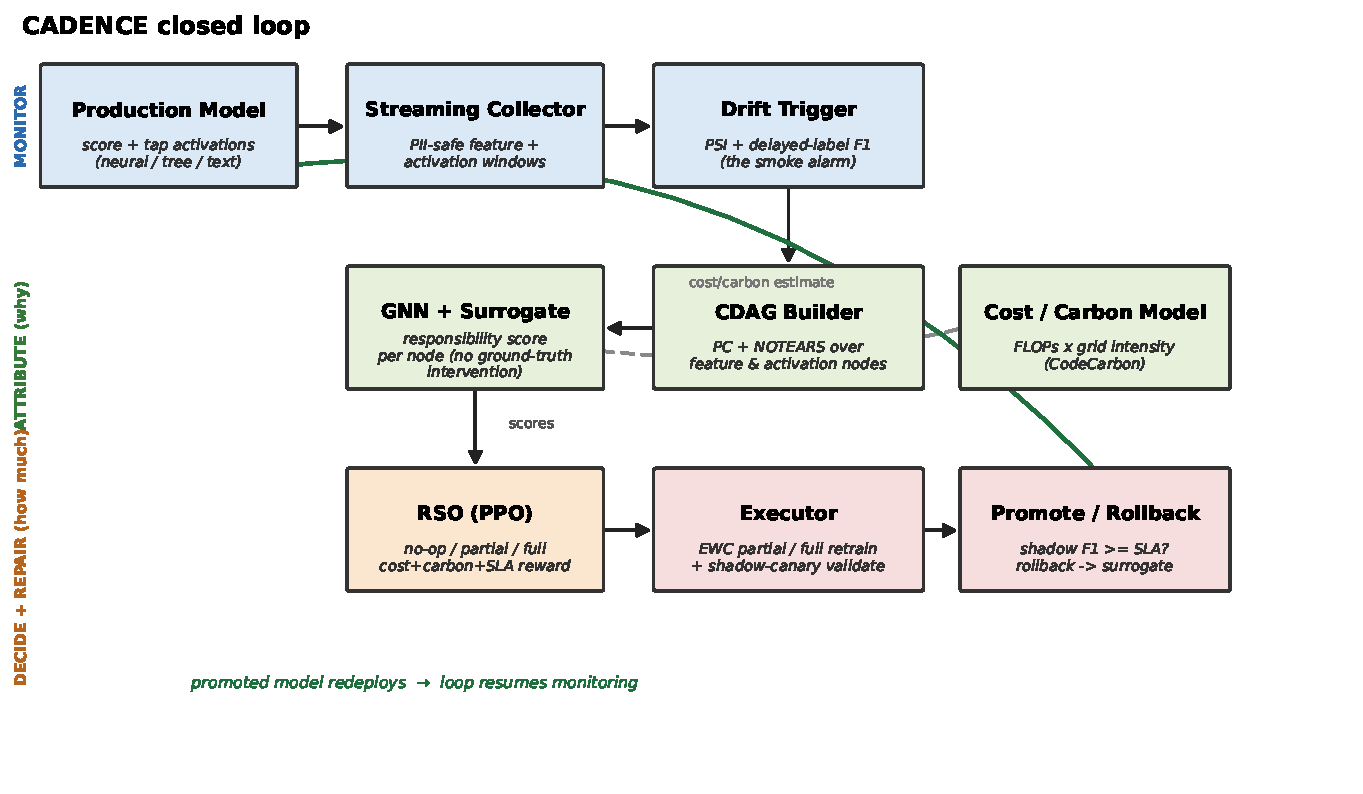
\includegraphics[width=\columnwidth]{fig_architecture.pdf}
\caption{CADENCE closed loop: monitor $\rightarrow$ attribute (CDAG + GNN +
counterfactual surrogate) $\rightarrow$ decide (cost-constrained scope) $\rightarrow$
repair (EWC partial/full + shadow validation) $\rightarrow$ redeploy.}
\label{fig:arch}
\end{figure}

\textbf{Attribution objective.} We do not claim graph identification. For a
candidate node $i$ we define the recovery of repairing it as
$R_i = P_i - P_{\text{cur}}$, where $P_i=\mathbb{E}[\mathrm{F1}(Y\mid do(\text{repair }i))]$.
A GNN produces a non-negative responsibility $r_i$ and an embedding $e_i$; a
surrogate predicts the post-repair performance $\hat P_i=g_\theta(e_i,[P_{\text{cur}},\text{sev}])$
and hence $\hat R_i=\hat P_i-P_{\text{cur}}$. Only $\hat R_i$ and $r_i$ feed the decision.

\textbf{Constrained decision (CMDP).} Scope selection over the action space
$\mathcal{A}=\{\textsc{no-op},\textsc{partial},\textsc{full}\}$ is a constrained
MDP. With target node $i^\ast=\arg\max_i r_i\hat R_i$, the partial action's
expected change is $\hat R_{i^\ast}$; among actions whose predicted post-repair
performance meets the SLA (predicted-feasible), the optimizer picks the least
compute cost $C(a)$, ranked by
\begin{equation}
J(a)=\mathbb{E}[\Delta\mathrm{F1}(a)]-w\,C(a)-\lambda\max(0,\mathrm{SLA}-\mathrm{F1}(a)),
\end{equation}
\begin{equation}
\lambda \leftarrow \mathrm{clip}\big(\lambda+\eta(\bar v-\delta),\,0,\,\lambda_{\max}\big),
\end{equation}
the dual $\lambda$ adapting to the realized violation rate $\bar v$ toward
target $\delta$. The optimizer is interchangeable (PPO~\cite{schulman2017} via
SB3~\cite{raffin2021}, contextual bandit, or greedy rule); Sec.~\ref{sec:sys}
shows PPO is not superior at this scale.

\textbf{Targeted repair.} An attributed node maps to a subnetwork: an
activation-cluster node to its tapped layer, a feature node to the input-facing
layer, multiple nodes to the union of scopes. The executor updates only that
parameter set, freezing the rest, under an EWC penalty
$\lambda_{\text{ewc}}\sum_j F_j(\theta_j-\theta_j^\ast)^2$ with diagonal Fisher
$F_j$; a concentration guard $\kappa=\max_i r_i/\sum_i r_i$ escalates to a full
retrain when responsibility is diffuse.

%=====================================================================
\section{Experimental Setup}\label{sec:setup}
%=====================================================================
\textbf{Pre-registration.} Before the confirmatory runs we fixed the Stage-1
policy-health gates and Stage-2 verdicts in a signed document, following the
preregistration rationale~\cite{nosek2018}; this prevents post-hoc metric
selection and lets us report negatives. \textbf{Data.} Synthetic drift with a
known root cause is injected into a Credit-Card-Fraud MLP across five scenarios;
real drift uses Elec2~\cite{harries1999}; cross-model generality uses LightGBM
(Give-Me-Some-Credit) and TF-IDF/logistic-regression (Yelp); forgetting uses
Split-MNIST~\cite{lecun1998}. Optimization uses Adam~\cite{kingma2015}.
\textbf{Protocol.} Results are over multiple seeds with paired Wilcoxon tests
and bootstrap confidence intervals; every value is regenerated from a versioned
ledger (dataset, seeds, config, hardware) and none is hand-entered.

%=====================================================================
\section{Results}\label{sec:res}
%=====================================================================
\subsection{H1: attribution beats correlation on contested drift}\label{sec:h1}
Reporting the easy/hard subsets separately (pooling dilutes the effect because
PSI is saturated on easy scenarios), on the \emph{contested} subset the
CDAG+GNN scorer lifts MRR from $0.097$ to $0.412$ and AUROC from $0.672$ to
$0.905$ ($p<0.001$ vs PSI, $n{=}10$; Fig.~\ref{fig:h1}, Table~\ref{tab:h1}).
Against stronger baselines the GNN \emph{dominates on AUROC} ($0.91$) over
input-gradient and permutation attribution (both $p\le0.032$), while a
counterfactual-permutation baseline is competitive on top-1/MRR
($p=0.42$)---so the GNN's clean, consistent win is ranking quality, honestly
reported.

\begin{figure}[t]
\centering
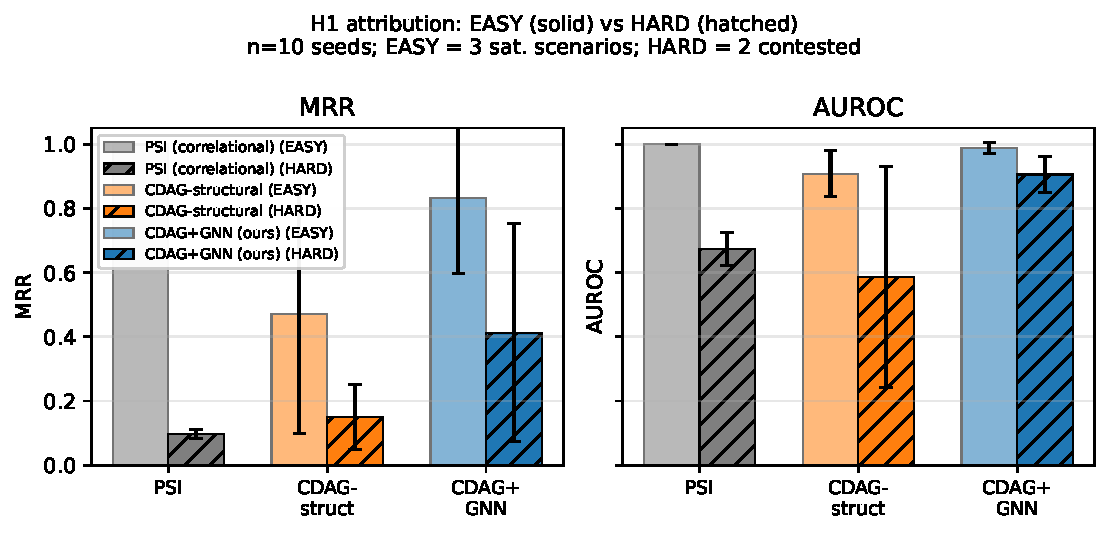
\includegraphics[width=0.82\columnwidth]{fig_h1_subset.pdf}
\caption{H1 ($n{=}10$). Solid: EASY (PSI-saturated); hatched: HARD (contested).
On HARD the CDAG+GNN beats both baselines on MRR and AUROC ($p<0.001$ vs PSI).}
\label{fig:h1}
\end{figure}

\begin{table}[t]
\centering\footnotesize
\caption{H1 on the HARD subset (mean; $n{=}10$). $p$: paired Wilcoxon (GNN
greater) on AUROC.}
\label{tab:h1}
\setlength{\tabcolsep}{5pt}
\begin{tabular}{@{}lcccc@{}}
\toprule
\textbf{Scorer} & \textbf{top-1} & \textbf{MRR} & \textbf{AUROC} & \textbf{$p$}\\
\midrule
PSI & $0.00$ & $0.097$ & $0.672$ & $<0.001$\\
Input-gradient & $0.00$ & $0.268$ & $0.517$ & $0.032$\\
Permutation & $\mathbf{0.50}$ & $\mathbf{0.517}$ & $0.293$ & $<0.001$\\
\textbf{CDAG+GNN} & $0.30$ & $0.450$ & $\mathbf{0.910}$ & ---\\
\bottomrule
\end{tabular}
\end{table}

\subsection{Counterfactual surrogate}\label{sec:sur}
Trained jointly with the GNN on sandbox interventions, the surrogate is
well-calibrated on held-out data ($R^2{=}0.888$, MAE $0.036$) and reaches
$R^2\!\approx\!0.9$ from $\sim\!50$--$100$ interventions---evidence it
\emph{amortizes} rather than memorizes. Its failure is reported honestly: a
mechanism-held-out test (train covariate drift, test unseen concept drift) gives
in-distribution MAE $0.004$ but out-of-distribution MAE $0.55$; cross-mechanism
generalization is an open problem, and an unrecoverable-drift guard halts
fruitless repair.

\subsection{H2: cost-constrained repair on real drift}\label{sec:h2}
On Elec2 the stream degrades from a train F1 of $0.84$ to an un-adapted $0.43$
(a genuine $41$-point drift; leakage-checked). Against a reactive-full baseline
CADENCE saves \textbf{69.1\%} of retraining compute for a $\mathbf{-1.66}$-point
F1 gap ($95\%$ CI $[-0.025,-0.009]$)---a Pareto-frontier point
(Fig.~\ref{fig:pareto}). A reduced learned-policy Stage~2 (3 seeds; documented
pre-registration amendment; full $10{\times}30$k run pending) strengthens this:
on the two \emph{recoverable} contested scenarios the learned scope selector
\emph{Pareto-dominates} PSI-full-retrain ($+0.02$ and $+0.09$ F1 at $66\%$ lower
compute); on an unrecoverable tail-flip all strategies fail equally. At $n{=}3$
the paired test is underpowered ($p{=}0.25$); we therefore report H2 as
PRACTICAL, not strict-dominance.

\begin{figure}[t]
\centering
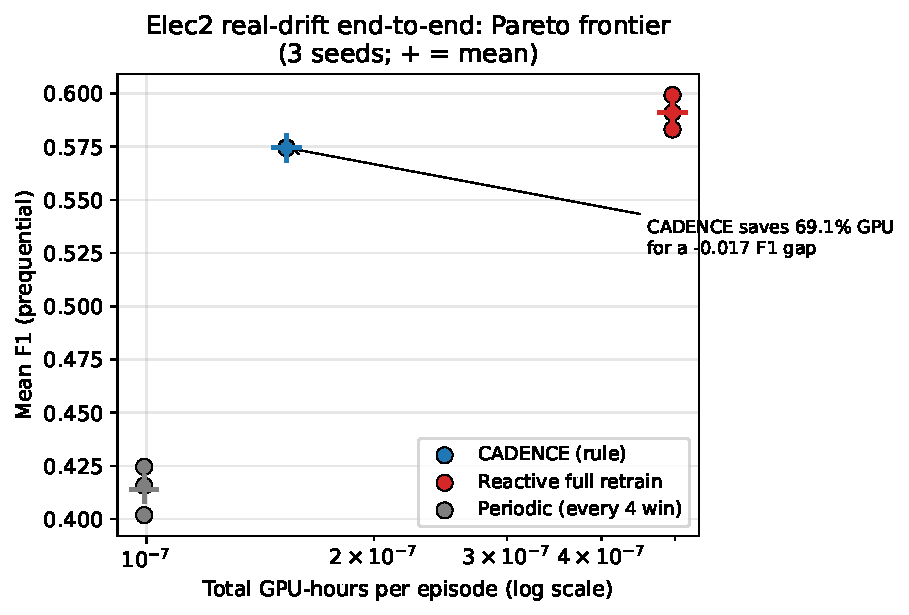
\includegraphics[width=0.82\columnwidth]{fig_elec2_pareto.pdf}
\caption{Real-drift Elec2 ($n{=}3$): CADENCE on the cost/F1 Pareto frontier
($-69.1\%$ GPU-hours vs reactive-full for a $-0.017$ F1 gap).}
\label{fig:pareto}
\end{figure}

\subsection{H3: targeted partial retraining reduces forgetting}\label{sec:h3}
On Split-MNIST (disjoint digit tasks) an EWC-regularized partial retrain
preserves the prior task almost perfectly (forgetting $-0.03$) while a naive
full retrain loses $39.5\%$; even against a fair full-with-replay baseline
partial retraining wins (paired Wilcoxon $p<0.001$, $n{=}10$;
Fig.~\ref{fig:h3}, Table~\ref{tab:h3}). Honestly, an isolation ablation shows
CDAG-guided layer targeting is \emph{tied} with random/gradient targeting on
forgetting: the win is EWC's, not causal layer selection's, on this benchmark.

\begin{figure}[t]
\centering
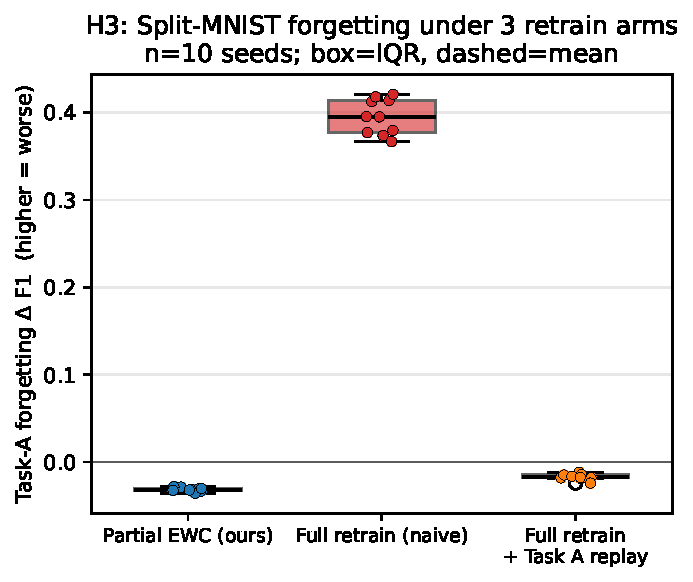
\includegraphics[width=0.82\columnwidth]{fig_h3_mnist_forget.pdf}
\caption{H3 Split-MNIST ($n{=}10$): partial-EWC preserves task A
(median $\approx-0.03$) vs naive-full loss $\approx0.40$; $p<0.001$.}
\label{fig:h3}
\end{figure}

\begin{table}[t]
\centering\footnotesize
\caption{H3 forgetting on Split-MNIST ($n{=}10$; lower is better, negative =
gain).}
\label{tab:h3}
\setlength{\tabcolsep}{6pt}
\begin{tabular}{@{}lccc@{}}
\toprule
\textbf{Retrain arm} & \textbf{Task-A forget} & \textbf{Task-B F1} & \textbf{$p$ vs ours}\\
\midrule
Naive full (no replay) & $+0.395$ & $0.990$ & $<0.001$\\
Full + replay (fair) & $-0.017$ & $0.979$ & $<0.001$\\
\textbf{Partial + EWC (ours)} & $\mathbf{-0.032}$ & $0.802$ & ---\\
\bottomrule
\end{tabular}
\end{table}

\subsection{System analysis and honest boundaries}\label{sec:sys}
Four measured system findings bound the claims. \emph{Overhead:} accounting for
CADENCE's own monitoring, CDAG, GNN and policy cost, the net saving is positive
only above a measured retrain-cost break-even ($\approx1.3$\,s); the headline is
a \emph{retraining}-compute saving. \emph{Scalability:} CDAG construction scales
$\approx O(n^{2.6})$ ($0.30$/$5.2$/$127$\,s at $30$/$100$/$300$ nodes), so we
build the graph only on a trigger and cap node count. \emph{Policy necessity:}
against no-op, always-partial, always-full and a greedy rule on the same
env/reward, PPO is competitive but \emph{not} superior ($p{=}0.29$ vs greedy);
we do not claim RL is necessary at a three-action scale. \emph{Diffuse cause:}
as $1{\to}10$ features co-drift, the concentration $\kappa$ falls monotonically
($0.94{\to}0.61$), correctly signalling escalation. A pre-registered Stage-1
diagnostic (7/8 policy-health gates) confirms the learned policy is
non-collapsed, exploring and constraint-satisfying---the substrate on which the
confirmatory run stands.

\subsection{Cross-model generality}
The identical loop runs over a neural MLP, a LightGBM ensemble and a TF-IDF/LR
text model; the \emph{architecture} is model-agnostic while the
\emph{partial-repair} mechanism needs internal layers (tree/linear adapters fall
back to full retrain by contract). On tree models at a realistic SLA CADENCE
still sits on the Pareto frontier ($50\%$ compute saved for a $0.007$ F1 cost).

%=====================================================================
\section{Limitations}\label{sec:lim}
%=====================================================================
Causal validity is shown on synthetic drift only (real drift is graded on
outcome; cross-mechanism transfer fails, Sec.~\ref{sec:sur}); H2's
strict-dominance form awaits the pre-registered $n{\ge}10$ learned-policy run;
PPO superiority and causal-targeting benefit are measured negatives at current
scale; graph construction is costly beyond $\sim\!100$ nodes; and carbon is
model-derived, so the headline is kept on compute. None of these undermine the
established H1, H3, surrogate-calibration, robustness or generality results.

%=====================================================================
\section{Conclusion}\label{sec:conc}
%=====================================================================
CADENCE reframes model maintenance from ``when to retrain'' to
``minimum-cost repair under a performance constraint,'' instantiated as one
closed loop over external-and-internal attribution, counterfactual benefit
prediction and cost-constrained scope selection. The core is established with
pre-registered, reproducible evidence---attribution beats correlation where the
problem is hard ($p<0.001$); targeted partial retraining eliminates forgetting
on a multi-task benchmark against a fair baseline ($p<0.001$); the surrogate is
well-calibrated. We are equally explicit about the frontier: the cost saving is
a reproducible practical Pareto win whose strict form is pending, and neither
PPO superiority nor causal layer targeting is established at this scale. Strong
claims where the evidence is strong, published protocols where it is not: this
separation makes the system both defensible and deployable.

%=====================================================================
% References — ASCENDING order of publication year.
%=====================================================================
\begin{thebibliography}{99}
\bibitem{mccloskey1989} M.\ McCloskey and N.\ J.\ Cohen, ``Catastrophic interference in connectionist networks: The sequential learning problem,'' \emph{Psychology of Learning and Motivation}, vol.\ 24, pp.\ 109--165, 1989.
\bibitem{lecun1998} Y.\ LeCun, L.\ Bottou, Y.\ Bengio, and P.\ Haffner, ``Gradient-based learning applied to document recognition,'' \emph{Proc.\ IEEE}, vol.\ 86, no.\ 11, pp.\ 2278--2324, 1998.
\bibitem{harries1999} M.\ Harries, ``SPLICE-2 comparative evaluation: Electricity pricing,'' Univ.\ New South Wales, Tech.\ Rep., 1999.
\bibitem{spirtes2000} P.\ Spirtes, C.\ Glymour, and R.\ Scheines, \emph{Causation, Prediction, and Search}, 2nd ed.\ MIT Press, 2000.
\bibitem{gama2004} J.\ Gama, P.\ Medas, G.\ Castillo, and P.\ Rodrigues, ``Learning with drift detection,'' in \emph{Brazilian Symp.\ Artif.\ Intell.\ (SBIA)}, 2004, pp.\ 286--295.
\bibitem{gama2014} J.\ Gama, I.\ \v{Z}liobait\.{e}, A.\ Bifet, M.\ Pechenizkiy, and A.\ Bouchachia, ``A survey on concept drift adaptation,'' \emph{ACM Comput.\ Surv.}, vol.\ 46, no.\ 4, pp.\ 1--37, 2014.
\bibitem{sculley2015} D.\ Sculley \emph{et al.}, ``Hidden technical debt in machine learning systems,'' in \emph{NeurIPS}, 2015.
\bibitem{kingma2015} D.\ P.\ Kingma and J.\ Ba, ``Adam: A method for stochastic optimization,'' in \emph{ICLR}, 2015.
\bibitem{kirkpatrick2017} J.\ Kirkpatrick \emph{et al.}, ``Overcoming catastrophic forgetting in neural networks,'' \emph{Proc.\ Natl.\ Acad.\ Sci.}, vol.\ 114, no.\ 13, pp.\ 3521--3526, 2017.
\bibitem{schulman2017} J.\ Schulman, F.\ Wolski, P.\ Dhariwal, A.\ Radford, and O.\ Klimov, ``Proximal policy optimization algorithms,'' \emph{arXiv:1707.06347}, 2017.
\bibitem{hamilton2017} W.\ L.\ Hamilton, R.\ Ying, and J.\ Leskovec, ``Inductive representation learning on large graphs,'' in \emph{NeurIPS}, 2017.
\bibitem{kipf2017} T.\ N.\ Kipf and M.\ Welling, ``Semi-supervised classification with graph convolutional networks,'' in \emph{ICLR}, 2017.
\bibitem{lundberg2017} S.\ M.\ Lundberg and S.-I.\ Lee, ``A unified approach to interpreting model predictions,'' in \emph{NeurIPS}, 2017.
\bibitem{lopezpaz2017} D.\ Lopez-Paz and M.\ Ranzato, ``Gradient episodic memory for continual learning,'' in \emph{NeurIPS}, 2017.
\bibitem{zheng2018} X.\ Zheng, B.\ Aragam, P.\ Ravikumar, and E.\ P.\ Xing, ``DAGs with NO TEARS: Continuous optimization for structure learning,'' in \emph{NeurIPS}, 2018.
\bibitem{nosek2018} B.\ A.\ Nosek, C.\ R.\ Ebersole, A.\ C.\ DeHaven, and D.\ T.\ Mellor, ``The preregistration revolution,'' \emph{Proc.\ Natl.\ Acad.\ Sci.}, vol.\ 115, no.\ 11, pp.\ 2600--2606, 2018.
\bibitem{lu2019} J.\ Lu, A.\ Liu, F.\ Dong, F.\ Gu, J.\ Gama, and G.\ Zhang, ``Learning under concept drift: A review,'' \emph{IEEE Trans.\ Knowl.\ Data Eng.}, vol.\ 31, no.\ 12, pp.\ 2346--2363, 2019.
\bibitem{rabanser2019} S.\ Rabanser, S.\ G\"unnemann, and Z.\ C.\ Lipton, ``Failing loudly: An empirical study of methods for detecting dataset shift,'' in \emph{NeurIPS}, 2019.
\bibitem{raffin2021} A.\ Raffin \emph{et al.}, ``Stable-Baselines3: Reliable reinforcement learning implementations,'' \emph{J.\ Mach.\ Learn.\ Res.}, vol.\ 22, no.\ 268, pp.\ 1--8, 2021.
\bibitem{delange2022} M.\ De Lange \emph{et al.}, ``A continual learning survey: Defying forgetting in classification tasks,'' \emph{IEEE Trans.\ Pattern Anal.\ Mach.\ Intell.}, vol.\ 44, no.\ 7, pp.\ 3366--3385, 2022.
\bibitem{paleyes2022} A.\ Paleyes, R.-G.\ Urma, and N.\ D.\ Lawrence, ``Challenges in deploying machine learning: A survey of case studies,'' \emph{ACM Comput.\ Surv.}, vol.\ 55, no.\ 6, pp.\ 1--29, 2022.
\end{thebibliography}

\end{document}
